\documentclass[10pt,twocolumn]{article}

\usepackage[letterpaper,margin=0.72in]{geometry}
\usepackage[T1]{fontenc}
\usepackage[utf8]{inputenc}
\usepackage{lmodern}
\usepackage{microtype}
\usepackage{amsmath,amssymb}
\usepackage{array}
\usepackage{booktabs}
\usepackage{graphicx}
\usepackage{listings}
\usepackage{tikz}
\usepackage{url}
\usetikzlibrary{arrows.meta,calc,positioning}

\raggedbottom
\emergencystretch=2em

\lstdefinelanguage{Jasmin}{
  morekeywords={fn,export,reg,mut,ptr,const,u32,u64,ui64,int,param,return,while,if,inline,require},
  sensitive=true,
  morecomment=[l]{//},
  morecomment=[s]{/*}{*/},
  morestring=[b]"
}

\lstdefinelanguage{Shell}{
  morekeywords={jasminc,jasmin-ct,sha256sum,diff,git},
  sensitive=true,
  morecomment=[l]{\#}
}

\lstset{
  basicstyle=\ttfamily\scriptsize,
  keywordstyle=\bfseries,
  columns=fullflexible,
  showspaces=false,
  showstringspaces=false,
  showtabs=false,
  keepspaces=true,
  breaklines=true,
  frame=single,
  framerule=0.2pt,
  xleftmargin=2pt,
  xrightmargin=2pt,
  aboveskip=4pt,
  belowskip=4pt
}

\newcommand{\haetae}{HAETAE}
\newcommand{\jasmin}{Jasmin}
\newcommand{\ct}{constant-time}
\newcommand{\sct}{speculative constant-time}
\newcommand{\Zq}{\mathbb{Z}_q}
\newcolumntype{P}[1]{>{\raggedright\arraybackslash}p{#1}}

% IEEE-style monochrome TikZ styles.
\tikzset{
  box/.style={
    rectangle, draw=black, fill=white, line width=0.45pt,
    minimum height=7mm, align=center,
    font=\scriptsize\sffamily, inner xsep=3pt, inner ysep=2pt
  },
  smallbox/.style={
    rectangle, draw=black, fill=white, line width=0.45pt,
    minimum height=6mm, align=center,
    font=\scriptsize\sffamily, inner xsep=2pt, inner ysep=1.5pt
  },
  checkerbox/.style={smallbox},
  ctbox/.style={smallbox, dashed},
  sctbox/.style={smallbox, densely dotted},
  artifactbox/.style={box, double, double distance=0.7pt},
  arrow/.style={-Stealth, line width=0.45pt, draw=black},
  dashedarrow/.style={-Stealth, line width=0.45pt, dashed, draw=black},
  note/.style={font=\tiny\sffamily, align=center, text=black}
}

\title{\vspace{-0.8em}An Analysis of \jasmin{} Safety and Constant-Time Verification for an NTT}
\author{Anonymous Submission}
\date{}

\begin{document}
\maketitle
\vspace{-1.1em}

\begin{abstract}
Low-level number-theoretic transform (NTT) implementations must be correct not
only as arithmetic programs, but also as machine-level artifacts whose memory
behavior and timing trace are disciplined.  This paper analyzes how the
\jasmin{} toolchain is used to verify safety and constant-time properties of a
scalar \haetae{} NTT implementation.  The analysis starts from the source shape
required by the checkers: loop bounds, table offsets, and pointer shapes must be
visible at the \jasmin{} level.  It then interprets three source-level checks:
\texttt{jasminc -checksafety} for defined execution, \texttt{jasmin-ct} for
regular branch/address constant time, and \texttt{jasmin-ct --speculative} for
the \jasmin{} SCT checker model.  Finally, it regenerates assembly and compares
it byte-for-byte with the submitted \path{hpoly.s}, so that source-level
evidence is tied to the assembly artifact.  The central result is a narrow but
replayable analysis claim: under typed pointer preconditions, the scalar NTT
exports are checked for in-bounds memory behavior and for public control-flow
and address traces independent of polynomial coefficients.  This claim
complements functional correctness proofs and does not establish full
microarchitectural leakage coverage or full \haetae{} signature security.
\end{abstract}

\section{Introduction}

NTT kernels are small enough to inspect by hand, but their implementation
security depends on details that are easy to overlook.  A loop counter used in
the wrong place may turn a public schedule into a secret-dependent memory
access.  A table bound that is obvious in a mathematical derivation may be
opaque to a compiler-side safety checker.  A wrapper that is constant time in
architectural execution may still need a speculation boundary before transient
pointer inputs are used for addressing.  These issues arise before the question
of functional correctness: a transform theorem is not an implementation claim
unless the compiled routine executes in a defined way and follows the intended
timing discipline.

This paper is an analysis of a methodology for checking those implementation
properties for the scalar \haetae{} NTT artifact written in \jasmin{}~\cite{Jasmin2017}.
The method is grounded in the files under \path{jasmin/}.  The exported entry
points are in \path{hpoly.jazz}; the stage-specialized NTT, inverse NTT, and
base-multiplication kernels are in \path{poly.jinc}; Montgomery multiplication
is in \path{reduce.jinc}; and parameters and twiddle tables are in
\path{params.jinc} and \path{zetas.jinc}.  The methodology uses the current
\jasmin{} checker workflow reflected in the 2026 framework material: source
safety checking, regular constant-time checking, and speculative
constant-time checking, followed by compilation to predictable assembly
~\cite{Jasmin2017,LastMile2020,JasminFramework2026}.

The methodology is deliberately narrower than a full implementation-correctness
proof.  It does not prove that the NTT computes the abstract transform; that is
the role of a companion functional proof in a tool such as EasyCrypt.  It also
does not prove full physical side-channel security or full \haetae{} signature
security.  Instead, it answers a prerequisite implementation question: how can
one structure a \jasmin{} NTT so that automatic checkers can prove safety,
regular \ct{}, and \sct{} properties, and how should those checker results be
interpreted?

\subsection{Theoretical Basis}

The theoretical basis of this methodology is a chain of conditional claims over
one \jasmin{} source program.  The first claim is semantic definedness: when an
exported routine is called with arguments satisfying its pointer preconditions,
execution terminates without leaving the language semantics.  The second claim
is regular constant-time noninterference: if two executions agree on public
inputs but differ in secret polynomial coefficients, then the observable
branch-and-address trace is the same.  The third claim is speculative
constant-time in the Jasmin SCT model: the same source is checked under a
Spectre-v1-style transient-execution discipline in which pointer security,
value security, and misspeculation state are tracked explicitly.  The final
claim is correspondence to the submitted artifact: the checked source is
compiled again and the resulting assembly is compared byte-for-byte with
\path{hpoly.s}.  These four claims are independent of, and strictly weaker
than, an algebraic proof that the NTT is functionally correct or a
cryptographic proof that \haetae{} is secure
~\cite{JasminFramework2026,Oliveira2022Thesis,JasminDocs}.

Safety is the defined-execution premise for every later argument.  A safe call
has a well-defined run from its initial memory and arguments to a final memory
and return values.  For this artifact, the relevant safety obligations are
termination of the fixed loops, in-bounds array indexing, valid and aligned
memory access, and valid arithmetic operations.  Typed pointers such as
\texttt{reg ptr u32[256]} give the checker a finite element type and index
shape, so source expressions such as \texttt{rp[i]} can be checked against the
256-word polynomial boundary.  They do not allocate external memory and do not
prove that arbitrary caller-provided addresses are valid.  Validity, allocation
size, mutability, and alignment remain ABI-side preconditions.  Therefore a
successful \texttt{jasminc -checksafety} run should be read as a conditional
semantic theorem: under the exported pointer preconditions, the source does not
perform an out-of-bounds access, invalid memory access, nonterminating loop, or
undefined primitive operation.

Regular constant time is a noninterference property over the leakage model used
by \texttt{jasmin-ct}.  The observable events are the program points where
secret data could influence timing: branch and loop conditions, memory
addresses, and array indices.  The
checker assigns security levels to expressions.  Public data may determine
control and addresses; secret data may flow through arithmetic and stored
values, but not into observable control or addressing positions.  For the NTT,
this gives the central invariant: stage numbers, loop counters, twiddle-table
offsets, and pointer bases form a public schedule, while loaded coefficients
and Montgomery products are secret values.  Changing the polynomial
coefficients may change register contents and stored coefficients, but it must
not change which branches are taken or which addresses are touched.

Speculative constant time is a separate, model-relative property.  At an
exported ABI boundary, pointer arguments are treated conservatively because the
processor may already be in a misspeculated state.  The wrappers therefore call
\texttt{\#init\_msf()}, which initializes the misspeculation-state discipline
and lowers to an assembly fence in the generated x86-64 code.  The SCT checker
then verifies that internal kernels operate with public pointer bases while the
pointed-to coefficients remain secret.  This rules out the Spectre-v1-style
pattern represented in the Jasmin SCT model for this call graph.  It is not a
claim about all transient-execution attacks, cache replacement behavior,
prefetching, power, electromagnetic leakage, frequency effects, or other
channels outside the checker model.

The source-to-assembly part is necessary because the checkers run on Jasmin
source, while the submitted artifact includes assembly.  The compiler is used
as the bridge: regenerate assembly from the checked source, hash it, and diff it
against \path{hpoly.s}.  If the files match, then the safety, CT, and SCT
claims are attached to the assembly under review for that compiler version and
that source revision.  If the source, compiler, target options, annotations, or
assembly change, the chain is broken and all evidence must be regenerated.

The ordering of these claims matters.  Safety comes first because CT and SCT
reasoning is meaningful only for executions that stay within the source
semantics.  Regular CT and SCT are separate because the latter tracks a
stronger transient-execution model and different pointer states.  Assembly
comparison comes last because it transfers the source-level evidence to the
submitted low-level file but does not prove a new binary-level theorem.

\begin{table}[t]
\centering
\scriptsize
\setlength{\tabcolsep}{3pt}
\begin{tabular}{P{0.34\columnwidth}P{0.56\columnwidth}}
\toprule
Principle & Consequence for this methodology \tabularnewline
\midrule
Defined execution & \texttt{-checksafety} is interpreted as a conditional proof
under exported pointer preconditions covering termination, bounds, valid memory,
alignment, and arithmetic validity. \tabularnewline
Regular CT noninterference & Secret coefficients may affect arithmetic values,
but branch conditions, loop conditions, memory addresses, and array indices must
be public. \tabularnewline
SCT model separation & The speculative result is confined to the Jasmin
Spectre-v1/selective-SLH checker model and is not stated as full
microarchitectural leakage freedom. \tabularnewline
Typed pointer discipline & Pointer types give element shape and index bounds to
the source checker; caller-side validity and alignment remain preconditions.
\tabularnewline
Source-to-assembly correspondence & Regeneration, hash comparison, and diff
comparison attach source-level checker evidence to \path{hpoly.s}. \tabularnewline
Claim separation & Safety, regular CT, SCT, source-to-assembly correspondence,
functional correctness, and cryptographic security are distinct claims.
\tabularnewline
\bottomrule
\end{tabular}
\caption{Direct theoretical basis used by the Jasmin NTT verification
methodology.}
\label{tab:method-theory-basis}
\end{table}

\paragraph{Contribution.}
The paper makes three contributions.
First, it states a concrete source-preparation discipline for NTT code: typed
polynomial pointers, stage-specialized loops, public table offsets, public
address expressions, and explicit exported wrapper annotations.  Second, it
gives a step-by-step checker methodology using \texttt{jasminc} and
\texttt{jasmin-ct}, including expected outcomes and failure interpretation.
Third, it explains how to tie source-level checker evidence to the generated
x86-64 assembly through regeneration, hash comparison, and diff comparison.

\paragraph{Paper organization.}
The paper proceeds from claim boundary to evidence.  Section~2 states the exact
routines and non-claims.  Sections~3 and~4 give the deductive and mathematical
CT arguments that justify why the checker obligations are the right ones for
this NTT.  Sections~5--9 describe the concrete Jasmin workflow and the source
shape that makes the obligations checkable.  Sections~10 and~11 record and
analyze the actual logs, while the final discussion states when the same method
would need stronger contracts or additional proofs.

\section{Verification Goal and Scope}

The checked artifact exports three scalar routines:
\[
\begin{array}{c}
  \texttt{poly\_ntt\_jazz},\quad \texttt{poly\_invntt\_jazz}\\
  \texttt{poly\_basemul\_jazz}.
\end{array}
\]
The first two implement the forward and inverse polynomial transforms used by
\haetae{} over \(q=64513\)~\cite{HAETAE2022}; the third performs coefficientwise
base multiplication in the NTT domain.  The methodology verifies the following
implementation-level properties.

\begin{table}[t]
\centering
\scriptsize
\setlength{\tabcolsep}{3pt}
\begin{tabular}{P{0.25\columnwidth}P{0.39\columnwidth}P{0.26\columnwidth}}
\toprule
Property & Methodological evidence & Non-claim \\
\midrule
Safety & \texttt{jasminc -checksafety} reports no safety violation for all
exports & Validity of arbitrary caller memory \\
Regular \ct{} & \texttt{jasmin-ct} accepts the source annotations & All
microarchitectural leakage channels \\
Speculative \ct{} & \texttt{jasmin-ct --speculative} accepts transient pointer
wrappers and MSF initialization & All Spectre variants or physical leakage \\
Assembly link & Regenerated assembly matches \path{hpoly.s} by hash and diff &
Hand-edited assembly correctness \\
\bottomrule
\end{tabular}
\caption{Methodology claims and boundaries.}
\label{tab:claims}
\end{table}

The methodology treats polynomial coefficients as secret and the NTT schedule as
public.  Public data include the selected routine, the loop bounds, stage
lengths, twiddle-table offsets, and pointer bases after the exported wrapper
boundary.  Secret data include coefficients loaded from polynomial arrays and
all arithmetic values derived from those coefficients.  The intended invariant
is that changing coefficients may change register contents and stored
coefficient values, but not the sequence of branches or memory addresses.

The result is conditional on ordinary low-level preconditions.  A type such as
\texttt{reg mut ptr u32[HAETAE\_N]} gives the checker a 256-word shape and
index discipline, but it does not prove that every possible caller pointer is a
valid object.  Validity, allocation, and alignment are caller or ABI
preconditions.  The safety check verifies that, under those preconditions, the
\jasmin{} source never steps outside its semantic domain.


\section{Mathematical Deduction for the Verification Method}

Let \(S\) be the \jasmin{} source file \path{jasmin/hpoly.jazz}, let \(A\)
be the submitted assembly file \path{hpoly.s}, and let \(F\) range over the
three exported routines.  For each exported routine \(f\in F\), let \(P_f\) be
its caller precondition: every pointer argument denotes allocated, aligned, and
sufficiently large memory matching the typed pointer shape in the source.  Let
\(\mathsf{Leak}_{\ct{}}(S,f,\sigma)\) be the regular Jasmin leakage trace of a
safe execution from initial state \(\sigma\), consisting of the observable
control-flow and address events checked by \texttt{jasmin-ct}.  Let
\(\sigma_0\equiv_{\mathsf{pub}}\sigma_1\) mean that two initial states agree on
all public inputs: routine choice, pointer bases, array extents, public tables,
loop bounds, and the public calling context.  The polynomial coefficients may
differ.

The deductive structure used by the paper has four premises.
\begin{enumerate}
  \item For every export \(f\in F\), \(P_f\Rightarrow
  \mathsf{Safe}(S,f)\).
  \item For every export \(f\in F\), if
  \(\sigma_0\equiv_{\mathsf{pub}}\sigma_1\), then
  \(\mathsf{Leak}_{\ct{}}(S,f,\sigma_0)=
  \mathsf{Leak}_{\ct{}}(S,f,\sigma_1)\).
  \item For every export \(f\in F\), \(\mathsf{SCT}_{\jasmin}(S,f)\).
  \item The regenerated assembly satisfies \(\mathsf{Compile}_{\jasmin}(S)=A\).
\end{enumerate}
From these premises the conclusion is that \path{hpoly.s} is the submitted
assembly for the checked source, and that under \(P_f\) the source-level
evidence establishes safety, regular CT, and Jasmin SCT for the exported scalar
NTT routines.

The first premise is discharged by \texttt{jasminc -checksafety}; the second by
\texttt{jasmin-ct}; the third by \texttt{jasmin-ct --speculative}; and the
fourth by regenerating assembly and comparing it with \path{hpoly.s}.  The rule
is conditional because it depends on the pointer preconditions and on the fixed
compiler/source pair recorded in the logs.  It is also intentionally
implementation-level: none of the premises states that the NTT formula is
algebraically correct, that base multiplication is functionally correct, or
that the full \haetae{} signature scheme is cryptographically secure.

\paragraph{Soundness reading.}
The four premises support the following theorem-shaped artifact claim.  If the
logs are fresh for the stated source revision and all checker commands exit
successfully, then every exported call satisfying \(P_f\) has defined
source-level execution; any two such calls with the same public inputs have the
same regular Jasmin branch/address leakage trace; the exported wrappers satisfy
the Jasmin SCT discipline for transient pointer inputs and secret pointed-to
values; and the submitted \path{hpoly.s} is the regenerated assembly for that
checked source.  Conversely, the claim no longer follows if the source,
annotations, compiler version, target options, assembly file, or pointer
preconditions change without regenerating the evidence.

\section{Mathematical Constant-Time Argument for the NTT Kernels}

The constant-time property of the scalar NTT implementation follows from a
schedule argument.  Let \(N=256\) and \(q=64513\).  A polynomial is an array
\(a=(a_0,\ldots,a_{255})\) of coefficient representatives over \(\Zq\).  The
coefficient representatives are treated as secret.  The routine name, pointer
bases, loop bounds, stage lengths, and twiddle-table positions are treated as
public.

Algebraically, each stage is a fixed linear transformation over \(\Zq\).  A
forward butterfly on positions \(i\) and \(k\) applies
\[
  (a_i,a_k)\longmapsto (a_i+\zeta_z a_k,\; a_i-\zeta_z a_k),
\]
and an inverse butterfly applies the corresponding inverse-stage operation
using the public inverse twiddle table and final public scaling factor.  Thus
the Jasmin program has the standard radix-two NTT butterfly graph: the graph
vertices are coefficient positions, the edges are public butterfly pairs, and
the edge labels are public twiddle-table entries.  The CT argument uses this
graph property directly.  It does not require coefficient values to be public,
and it does not by itself prove that the twiddle table is the intended table;
that table-level algebraic fact belongs to functional-correctness validation,
whereas the present checker evidence proves that the chosen table is used
through a public, coefficient-independent schedule.

For a forward stage with public butterfly length
\(\ell\in\{128,64,32,16,8,4,2,1\}\), define \(B=N/(2\ell)\).  The Jasmin
helper for that stage iterates over public counters
\[
  0\le b < B,
  \qquad 0\le j < \ell,
\]
and computes
\[
  i=b(2\ell)+j,
  \qquad k=i+\ell,
  \qquad z=B+b.
\]
Hence \(0\le i<256\), \(0\le k<256\), and the accessed locations
\(\texttt{rp}[i]\), \(\texttt{rp}[k]\), and \(\texttt{jzetas}[z]\) are functions
only of public quantities.  The butterfly then performs the arithmetic
\[
  t = \zeta_z a_k,
  \qquad a_i^{+} = a_i + t,
  \qquad a_k^{+} = a_i - t,
\]
where multiplication is the fixed Montgomery multiplication implemented by
\texttt{\_\_fqmul}.  The values \(a_i\), \(a_k\), \(t\), \(a_i^{+}\), and
\(a_k^{+}\) may be secret, but they are not used to choose a branch, loop
bound, array index, or memory address.

The inverse stages have the same trace structure.  For a public length
\(\ell\in\{1,2,4,8,16,32,64,128\}\), the counters again determine
\(i=b(2\ell)+j\) and \(k=i+\ell\).  The exact inverse-stage table base used
by the source is \(I_\ell=256-N/\ell\), so the twiddle index is
\(z=I_\ell+b\).  Hence the inverse twiddle address is also a public
affine function of the block counter, and the final scaling loop touches
\(\texttt{rp}[j]\) for the public counter \(0\le j<N\).  Its arithmetic has the
form
\[
  a_i^{+} = a_i + a_k,
  \qquad a_k^{+} = \zeta_z(a_i-a_k),
\]
followed by public-schedule scaling.  Again, secret coefficients affect only
arithmetic data, not the trace.

Base multiplication is even more direct.  For public \(0\le i<N\), it reads
\(\texttt{ap}[i]\) and \(\texttt{bp}[i]\), computes
\(\texttt{\_\_fqmul}(a_i,b_i)\), and writes \(\texttt{rp}[i]\).  The accessed
locations are determined by the public index \(i\) and public pointer bases;
the loaded coefficients and product are secret arithmetic values.

Therefore, for any two safe executions with the same public inputs and possibly
different coefficients, the forward NTT, inverse NTT, and base multiplication
visit the same sequence of code branches and memory addresses.  This is the
mathematical invariant that the Jasmin CT annotations express and that
\texttt{jasmin-ct} checks syntactically.  The recorded CT result is thus not a
black-box observation: it is the tool confirmation of the public-schedule
argument above, within the Jasmin default branch/address leakage model used by
the artifact.

\section{Methodology Overview}

Figure~\ref{fig:pipeline} shows the verification pipeline.  The method starts
from one \jasmin{} source entry point, \path{jasmin/hpoly.jazz}.  That file
imports the kernel code and exposes the three ABI-level wrappers.  The same
source is then used for all checker runs; there is no separate safety-only or
CT-only source.

\begin{figure}[t]
\centering
\resizebox{\columnwidth}{!}{%
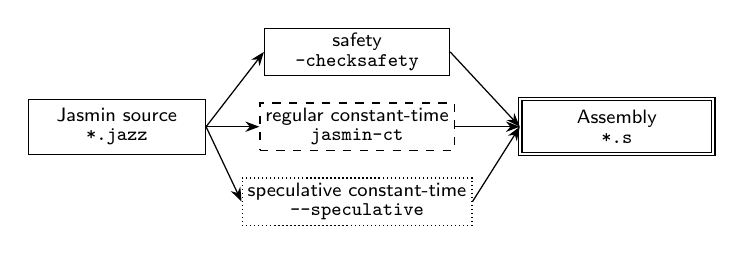
\begin{tikzpicture}[x=1cm,y=1cm]
  \node[box, minimum width=2.25cm] (src) at (0,0)
    {\jasmin{} source\\[-1pt]\texttt{*.jazz}};
  \node[checkerbox, minimum width=2.35cm] (safe) at (3.05,0.95)
    {safety\\[-1pt]\texttt{-checksafety}};
  \node[ctbox, minimum width=2.35cm] (ct) at (3.05,0)
    {regular \ct{}\\[-1pt]\texttt{jasmin-ct}};
  \node[sctbox, minimum width=2.35cm] (sct) at (3.05,-0.95)
    {speculative \ct{}\\[-1pt]\texttt{--speculative}};
  \node[artifactbox, minimum width=2.45cm] (asm) at (6.35,0)
    {Assembly\\[-1pt]\texttt{*.s}};
  % \node[box, minimum width=2.2cm] (diff) at (9.25,0)
  %   {compare\\[-1pt]\texttt{hpoly.s}};

  \draw[arrow] (src.east) -- (safe.west);
  \draw[arrow] (src.east) -- (ct.west);
  \draw[arrow] (src.east) -- (sct.west);
  \draw[arrow] (safe.east) -- (asm.west);
  \draw[arrow] (ct.east) -- (asm.west);
  \draw[arrow] (sct.east) -- (asm.west);
  % \draw[arrow] (asm.east) -- (diff.west);
  % \node[note] at (6.35,-1.10) {source checks are meaningful for the submitted
  %   assembly only after regeneration agrees};
\end{tikzpicture}}
\caption{Verification pipeline.}
\label{fig:pipeline}
\end{figure}

The pipeline has five operational steps.

\begin{enumerate}
  \item Record the toolchain version with \texttt{jasminc -version}.
  \item Run the \jasmin{} safety checker using \texttt{jasminc -checksafety}.
  \item Run the regular \ct{} checker using \texttt{jasmin-ct}.
  \item Run the speculative checker using \texttt{jasmin-ct --speculative}.
  \item Regenerate assembly and compare it with the submitted \path{hpoly.s}.
\end{enumerate}

The steps are intentionally run on the same source file.  If the source, the
compiler version, the target options, or the submitted assembly changes, all
evidence must be regenerated.

\section{Preparing the Jasmin Source}

Automatic checking is not only a command-line activity.  The source must expose
the relevant invariants in a form the checkers can use.  For the scalar
\haetae{} NTT, the central design choice is stage specialization.  Rather than
write one loop with a mutable stage length, the implementation uses fixed
helpers for lengths
\[
  128,64,32,16,8,4,2,1
\]
in the forward transform and the reverse order in the inverse transform.  The
source organization is small enough to audit directly, but each file has a
different verification role.

\begin{table}[t]
\centering
\scriptsize
\setlength{\tabcolsep}{3pt}
\begin{tabular}{P{0.25\columnwidth}P{0.30\columnwidth}P{0.35\columnwidth}}
\toprule
File & Artifact role & Verification relevance \tabularnewline
\midrule
\path{hpoly.jazz} & Exported ABI wrappers & Contains \ct{} and \sct{}
annotations and the \texttt{\#init\_msf()} boundary. \tabularnewline
\path{poly.jinc} & NTT, inverse NTT, and base multiplication kernels & Exposes
stage-specialized public loops and public index expressions. \tabularnewline
\path{reduce.jinc} & Montgomery multiplication and reduction & Keeps coefficient
arithmetic in fixed straight-line helper code. \tabularnewline
\path{params.jinc}, \path{zetas.jinc} & Public parameters and twiddle tables &
Fixes \(N=256\), \(q=64513\), and public table addresses. \tabularnewline
\path{hpoly.s} & Submitted assembly artifact & Must match regenerated assembly
before source-level evidence applies. \tabularnewline
\bottomrule
\end{tabular}
\caption{Source files and their verification roles.}
\label{tab:source-roles}
\end{table}

The first forward helper illustrates the shape.

\begin{lstlisting}[language=Jasmin,caption={Stage-specialized forward helper.},label={lst:stage}]
fn _poly_ntt_stage_128(reg mut ptr u32[HAETAE_N] rp)
    -> reg ptr u32[HAETAE_N] {
  reg ptr u32[256] zetasp;
  reg ui64 block j start idx offset;
  reg u32 zeta t s coeff;

  zetasp = jzetas;
  block = 0;
  while (block < 1) {
    zeta = zetasp[1 + block];
    start = block;
    start <<= 8;
    j = 0;
    while (j < 128) {
      idx = j;
      idx += start;
      s = rp[idx];
      offset = idx;
      offset += 128;
      coeff = rp[offset];
      t = __fqmul(zeta, coeff);
      coeff = s;
      coeff -= t;
      rp[offset] = coeff;
      s += t;
      rp[idx] = s;
      j += 1;
    }
    block += 1;
  }
  return rp;
}
\end{lstlisting}

This shape helps both safety and \ct{} checking.  The bounds checker sees
literal facts such as \(\texttt{block}<1\), \(\texttt{j}<128\), and
\(\texttt{offset}=\texttt{idx}+128\).  The timing checker sees that all
addresses are computed from pointer bases, public counters, and public stage
constants.  The loaded coefficient values \texttt{s} and \texttt{coeff} are
secret, but they are used only in arithmetic and stores.

The exported wrappers carry the security boundary.  For example, the forward
wrapper is annotated for both regular and speculative checking.

\begin{lstlisting}[language=Jasmin,caption={Exported wrapper annotation.},label={lst:wrapper}]
#[ct = "rp -> rp"]
#[sct = "{ ptr: transient, val: secret } ->
         { ptr: public, val: secret }"]
export
fn poly_ntt_jazz(reg mut ptr u32[HAETAE_N] rp)
    -> reg ptr u32[HAETAE_N] {
  _ = #init_msf();
  rp = _poly_ntt(rp);
  return rp;
}
\end{lstlisting}

The regular \ct{} annotation states the source-level information-flow policy.
The SCT annotation separates pointer security from pointed-to-value security:
the wrapper receives a transient pointer at the ABI boundary, initializes the
microarchitectural speculation state, then calls the internal kernel with a
public pointer base while preserving secret coefficient values.

\section{Safety Checking}

The safety checker is invoked through \texttt{jasminc}.  The command used for
this artifact is:

\begin{lstlisting}[language=Shell,caption={Safety checker command.},label={lst:safetycmd}]
jasminc -checksafety -o /tmp/hpoly-safe.s jasmin/hpoly.jazz
\end{lstlisting}

The expected output contains \texttt{No Safety Violation} for each export:
\path{poly_ntt_jazz}, \path{poly_invntt_jazz}, and
\path{poly_basemul_jazz}.  The assembly output file is incidental here; the
purpose of the command is to run the safety analysis while compiling.

\begin{table}[t]
\centering
\scriptsize
\setlength{\tabcolsep}{3pt}
\begin{tabular}{P{0.28\columnwidth}P{0.35\columnwidth}P{0.27\columnwidth}}
\toprule
Obligation & Source fact used & Example \\
\midrule
Polynomial bounds & Typed pointer has 256-word shape; index is public and
bounded & \texttt{j < 128} implies \texttt{j + 128 < 256} \\
Twiddle bounds & Stage helper fixes table offset and block range & First
stage reads \texttt{jzetas[1 + block]} with \texttt{block < 1} \\
Memory mutability & Output pointer is mutable; inputs to base multiplication
are const & \texttt{rp[i]} is written, \texttt{ap[i]} and \texttt{bp[i]} are
read \\
Arithmetic definedness & Montgomery helper uses explicit casts, signed
shifts, and word widths & \texttt{\_\_fqmul} calls Montgomery reduction \\
\bottomrule
\end{tabular}
\caption{Safety obligations and source facts.}
\label{tab:safety}
\end{table}

The output must be read conditionally.  A successful safety run does not prove
that arbitrary machine addresses supplied by a caller are valid.  Instead, it
proves that if the caller satisfies the typed pointer preconditions, then the
source execution stays within the declared arrays and uses primitive operations
within the \jasmin{} semantics.  This conditional reading is essential for
cryptographic low-level code: safety is the definedness layer on which both
functional and timing arguments rely.

\section{Regular Constant-Time Checking}

The regular \ct{} checker is run with:

\begin{lstlisting}[language=Shell,caption={Regular constant-time checker command.},label={lst:ctcmd}]
jasmin-ct jasmin/hpoly.jazz
\end{lstlisting}

For this artifact, success is silent: the command produces no diagnostic output
and exits with status 0.  That silence should not be interpreted as a manual
inspection result.  The checker has traversed the program under the exported
security annotations and verified that expressions reaching observable timing
positions are public in the checker model.

The leakage model used here treats branch conditions, loop guards, memory
addresses, and array indices as observable.  The methodology therefore enforces the following
discipline.

\begin{table}[t]
\centering
\scriptsize
\setlength{\tabcolsep}{3pt}
\begin{tabular}{P{0.33\columnwidth}P{0.27\columnwidth}P{0.30\columnwidth}}
\toprule
Program component & Label expected & Reason \\
\midrule
Loop bounds and counters & Public & Determine control-flow length \\
Twiddle-table offsets & Public & Determine table address sequence \\
Pointer bases after wrapper boundary & Public & Determine memory addresses \\
Loaded polynomial coefficients & Secret & Contain input-dependent data \\
Montgomery products and sums & Secret & Derived from coefficients \\
\bottomrule
\end{tabular}
\caption{Regular \ct{} labeling discipline.}
\label{tab:ctlabels}
\end{table}

The base-multiplication kernel is the simplest instance.  It performs a public
256-iteration loop, reads \texttt{ap[i]} and \texttt{bp[i]}, computes
\texttt{\_\_fqmul(a,b)}, and stores \texttt{rp[i]}.  The values \texttt{a},
\texttt{b}, and the product are secret; the index \texttt{i} and the touched
locations are public.  The NTT stages use the same discipline with a nested
public schedule.

\section{Speculative Constant-Time Checking}

Speculative checking is run with:

\begin{lstlisting}[language=Shell,caption={Speculative checker command.},label={lst:sctcmd}]
jasmin-ct --speculative jasmin/hpoly.jazz
\end{lstlisting}

The checker prints inferred security types for the internal and exported
routines.  For the exported NTT wrappers, the important shape is:
\[
\begin{array}{c}
\{\texttt{ptr}:\texttt{transient},\ \texttt{val}:\texttt{secret}\}\\
\to\\
\{\texttt{ptr}:\texttt{public},\ \texttt{val}:\texttt{secret}\}.
\end{array}
\]
For \path{poly_basemul_jazz}, all three pointer arguments have the same
transient-pointer, secret-value input shape, and the result is a public pointer
to secret values.

The key source operation is \texttt{\#init\_msf()}, shown in
Listing~\ref{lst:wrapper}.  In the generated x86-64 assembly used here, each
exported wrapper begins with an \texttt{lfence}.  Methodologically, this means
the exported boundary is part of the proof: ABI-provided pointer bases are not
assumed public for speculative addressing until the wrapper has initialized the
speculation state.  After that point, internal kernels use public pointer bases
and public counters for addressing, while coefficient values remain secret.

This is a model-relative claim.  It is a \jasmin{} SCT/Spectre-v1-style checker
claim for this source and this call graph.  It is not a measurement claim about
power, electromagnetic leakage, frequency scaling, cache replacement state, or
all speculative-execution variants.

\section{Connecting Source Checks to Assembly}

The source-level checks are meaningful for the submitted assembly only if the
assembly is the compiler output of the checked source.  The methodology
therefore includes assembly regeneration and comparison.

\begin{lstlisting}[language=Shell,caption={Assembly regeneration and comparison.},label={lst:asmcmd}]
jasminc jasmin/hpoly.jazz -o /tmp/hpoly-after.s
sha256sum hpoly.s /tmp/hpoly-after.s
diff -u hpoly.s /tmp/hpoly-after.s
\end{lstlisting}

The expected result is that the hashes match and the diff is empty.  This step
does not create a separate binary-analysis proof.  It establishes that the
assembly file under review is the assembly emitted by the same \jasmin{} source
that passed the safety and timing checks.  If \path{hpoly.s} is edited by hand,
compiled with a different toolchain, or generated with different target
options, the source-to-assembly evidence must be regenerated.

\section{Reproducibility Evidence}

The method is intended to be auditable.  A complete reproduction record should
include the tool version, source revision, checker logs, compilation log, and
assembly comparison.  The following command sequence records the evidence used
by the artifact.

\begin{lstlisting}[language=Shell,caption={Commands for refreshing reproducibility logs.},label={lst:logcmd}]
jasminc -version > paper/logs/jasminc-version.log
git rev-parse --short HEAD > paper/logs/git-revision.log
jasminc -checksafety -o /tmp/hpoly-safe.s jasmin/hpoly.jazz \
  > paper/logs/jasmin-checksafety.log 2>&1
jasmin-ct jasmin/hpoly.jazz > paper/logs/jasmin-ct.log 2>&1
jasmin-ct --speculative jasmin/hpoly.jazz \
  > paper/logs/jasmin-ct-speculative.log 2>&1
jasminc jasmin/hpoly.jazz -o /tmp/hpoly-after.s \
  > paper/logs/jasmin-compile.log 2>&1
sha256sum hpoly.s /tmp/hpoly-after.s > paper/logs/assembly-sha256.log
diff -u hpoly.s /tmp/hpoly-after.s > paper/logs/assembly-diff.log
\end{lstlisting}

The command exit status is part of the evidence even when the redirected log is
empty or whitespace-only.  In particular, an empty or blank \path{jasmin-ct.log}, empty
\path{jasmin-compile.log}, or empty \path{assembly-diff.log} should be read as
success only together with exit status 0.  A future archival run can make this
fully explicit by storing a small status file for each command, but the logical
claim in this paper always depends on successful command completion as well as
on the file contents.

Table~\ref{tab:logs} summarizes the expected interpretation of those logs.

\begin{table}[t]
\centering
\scriptsize
\setlength{\tabcolsep}{3pt}
\begin{tabular}{P{0.35\columnwidth}P{0.55\columnwidth}}
\toprule
Log & Expected interpretation \\
\midrule
\path{jasminc-version.log} & Records the \jasmin{} compiler version. \\
\path{jasmin-checksafety.log} & Reports no safety violation for all three
exports. \\
\path{jasmin-ct.log} & May be empty or blank when regular \ct{} checking succeeds. \\
\path{jasmin-ct-speculative.log} & Shows transient-pointer exported wrappers
and public internal pointer bases over secret values. \\
\path{jasmin-compile.log} & May be empty when assembly generation succeeds. \\
\path{assembly-sha256.log} and \path{assembly-diff.log} & Show that regenerated
assembly matches \path{hpoly.s}. \\
\bottomrule
\end{tabular}
\caption{Reproducibility evidence.}
\label{tab:logs}
\end{table}


\section{Analysis of Verification Results}

The recorded logs turn the methodology into an auditable artifact claim rather
than a checklist of commands.  The run was performed with \jasmin{} compiler
\texttt{2026.03.0} and repository revision \texttt{f0e1399}, as recorded in
\path{jasminc-version.log} and \path{git-revision.log}.  These two facts are
part of the result because both the source and the checker implementation are
inputs to the claim.  The auxiliary logs also expose useful audit facts:
\path{jasmin-ct.log} is blank apart from a newline, \path{jasmin-compile.log}
and \path{assembly-diff.log} are zero-byte files, and
\path{assembly-sha256.log} records the same SHA-256 digest for both
\path{hpoly.s} and \path{/tmp/hpoly-after.s}.

The most important \texttt{jasminc} result is the safety log.  It analyzes the
three exported functions independently and prints \texttt{No Safety Violation}
for \path{poly_ntt_jazz}, \path{poly_invntt_jazz}, and
\path{poly_basemul_jazz}.  For the two in-place NTT routines, the only listed
symbolic memory name is \texttt{mem\_rp}; for base multiplication the listed
names are \texttt{mem\_rp}, \texttt{mem\_ap}, and \texttt{mem\_bp}.  In all
three cases the reported ranges are \([0,0]\) with equality relations such as
\(\texttt{mem\_rp}=0\).  In light of the \jasmin{} safety documentation, this
should be read carefully: the checker did not synthesize an additional
variable-length memory-region obligation for this fixed-size typed-pointer
source, but the result is still conditional on the exported typed pointer
arguments denoting valid and suitably aligned caller-provided memory.  It is
not a proof that arbitrary machine addresses are safe.

The regular \ct{} log is blank apart from a newline.  This is meaningful only together with the
successful command completion: \texttt{jasmin-ct} reports no failed typing
obligation for the exported annotations.  The analysis consequence is that, in
the Jasmin CT type-system model, coefficient values may remain secret, but the
observed control-flow and memory-address expressions are public.  This matches
the intended NTT separation between public schedule data and secret polynomial
coefficients.

The speculative \ct{} log is verbose and should be used to inspect the exported
security boundary.  It records internal stage helpers as \texttt{modmsf}
routines whose pointer component is public and whose value component is secret.
For the three exported wrappers it records transient pointer inputs and public
pointer outputs over secret values.  For example, \path{poly\_ntt\_jazz} and
\path{poly\_invntt\_jazz} have the shape
\(\{\texttt{ptr}:\texttt{transient},\texttt{val}:\texttt{secret}\}\to
\{\texttt{ptr}:\texttt{public},\texttt{val}:\texttt{secret}\}\), while
\path{poly\_basemul\_jazz} applies the same input discipline to its three
pointers.  This is exactly the wrapper pattern justified by
\texttt{\#init\_msf}: ABI-entering pointers are treated conservatively at the
boundary, then internal kernels operate with public pointer bases and secret
coefficient values.

The remaining \texttt{jasminc} evidence links those source-level results to the
submitted assembly.  \path{jasmin-compile.log} is empty, which records
successful assembly regeneration without diagnostics.  \path{assembly-diff.log}
is also empty, and \path{assembly-sha256.log} gives the same SHA-256 digest,
for both \path{hpoly.s} and \path{/tmp/hpoly-after.s}.  Therefore the checked
source and the assembly file submitted with the artifact are byte-for-byte
connected for this toolchain run.

\begin{table}[t]
\centering
\scriptsize
\setlength{\tabcolsep}{3pt}
\begin{tabular}{P{0.25\columnwidth}P{0.30\columnwidth}P{0.35\columnwidth}}
\toprule
Evidence & Observed log result & Analysis consequence \tabularnewline
\midrule
Tool and source version & \texttt{Jasmin Compiler 2026.03.0}; revision
\texttt{f0e1399} & The claim is tied to a concrete checker/compiler and source
snapshot. \tabularnewline
Safety & Three exported functions report \texttt{No Safety Violation} & The
source has defined execution under the typed-pointer caller preconditions.
\tabularnewline
Regular \ct{} & Blank \path{jasmin-ct.log} after successful execution & No
regular CT typing obligation failed for the exported annotations.
\tabularnewline
Speculative \ct{} & Exported wrappers type transient pointers to public
pointers over secret values & The SCT boundary matches the intended
\texttt{\#init\_msf}-based wrapper discipline. \tabularnewline
Assembly regeneration & Empty compile and diff logs; matching SHA-256 hashes &
\path{hpoly.s} is the regenerated assembly for the checked source.
\tabularnewline
\bottomrule
\end{tabular}
\caption{Analysis of the recorded verification logs.}
\label{tab:results-analysis}
\end{table}

The checks should be rerun after any change to \path{hpoly.jazz},
\path{poly.jinc}, \path{reduce.jinc}, \path{params.jinc}, \path{zetas.jinc},
\path{hpoly.s}, the \jasmin{} compiler version, or target compiler options.
They should also be reviewed manually if a patch introduces raw memory
operations, new exports, changed \ct{} or \sct{} annotations, data-dependent
branches, coefficient-indexed tables, or declassification.

\section{Discussion and Limitations}

The methodology is effective here because the scalar NTT is structurally
regular.  Stage-specialized helpers expose small integer facts to the safety
checker.  The CT proof matches the programmer's informal discipline: counters
and table offsets are public, coefficients and derived arithmetic values are
secret.  The exported wrappers provide one clear speculation boundary, and the
internal kernels do not introduce additional transient pointer boundaries.

The method is less informative if applied blindly to code with data-dependent
loop termination, raw pointer arithmetic, complicated heap structure, or
declassification.  In such cases, a passing checker result may require
additional explanation, or the code may need contracts and manual proof support.
The 2026 \jasmin{} material describes newer modular safety-check directions for
larger programs~\cite{JasminFramework2026}.  This artifact intentionally uses
\texttt{jasminc -checksafety} because the scalar NTT has no symbolic heap
allocation, no source stack arrays, and no secret-dependent loop bounds.

The methodology is also separate from cryptographic-security preservation in
the sense of recent compiler-security work for \jasmin{}
~\cite{ArranzOlmos2025JasminSecurity}.  That line of work studies preservation
of higher-level cryptographic security properties through the compiler
front-end.  The method described here supplies a lower implementation layer:
defined execution, public branch/address traces, and source-to-assembly
correspondence for the scalar NTT artifact.

\section{Conclusion}

This paper analyzed a methodology for verifying safety and constant-time
properties of a \jasmin{} NTT implementation.  The analysis has three parts:
shape the source so that checker obligations are explicit, interpret the
safety, regular \ct{}, and speculative \ct{} checker outputs for the same
exported source, and
tie those source-level results to the submitted assembly by regeneration and
comparison.  Applied to the scalar \haetae{} NTT, this yields a replayable
artifact claim: under typed pointer preconditions, the exported scalar routines
execute safely and have branch and memory-address traces independent of secret
polynomial coefficients in the \jasmin{} checker models.  This is the
implementation-side discipline that functional proofs and higher-level
cryptographic arguments need before they can be read as claims about generated
low-level code.

\bibliographystyle{abbrv}
\bibliography{refs}

\end{document}
